\documentclass[11pt]{article}
\usepackage[margin=2cm]{geometry}
\usepackage[T1]{fontenc}
\usepackage{lmodern}
\usepackage{booktabs}
\usepackage{longtable}
\usepackage{graphicx}
\usepackage{array}
\usepackage{caption}
\usepackage{float}
\usepackage{minted}
\usepackage[hidelinks]{hyperref}

% keep the generated tables where they are \input, next to their discussion
\floatplacement{table}{H}
\renewcommand{\arraystretch}{1.15}
\setlength{\parskip}{0.5em}
\setlength{\parindent}{0pt}

\title{CS4372 Assignment 4: A Tale of Two Cities}
\author{N. Ohayon Rozanes}
\date{\today}

\begin{document}
\maketitle

\section*{Data}

All four tasks use Charles Dickens' A Tale of Two Cities, taken from Project
Gutenberg and split into chapter. In total, there are 45 chapters
across three books. The novel was chosen because the BookSum
dataset (\texttt{kmfoda/\allowbreak booksum}) has reference summaries
at the chapter level, and Project Gutenberg also has a Spanish translation
by Gregorio Lafuerza with the same 45-chapter structure. The
Gutenberg chapters match BookSum's chapter text to within 20 words
for every chapter. All models were run on a Google Colab T4 GPU. Each
task is split into a method, evaluation, and discussion section.

%-------------------------------------------------------------------------------
\section{Summarization}

\textbf{Method.} Each chapter was summarized with
facebook's bart-large-cnn. This was a BART model fine tuned to
summarize CNN articles. BART reads at most 1024 tokens and every
chapter is longer (1,288 to 7,866 tokens, median 3,585), so each
chapter was split into equal chunks of at most 1,000 tokens.
Each chunk was decoded with beam search, tuned to give a similar
output to BookSum's reference summary.

\textbf{Evaluation.} BookSum has 4 to 6 reference summaries per
chapter, written by different study guides. Each generated summary
was scored against every reference for its chapter, keeping the best
F1 for ROUGE-1, ROUGE-2 and ROUGE-L and for BERTScore (rescaled with
its baseline, so that 0 is roughly the similarity of two unrelated sentences).

\begin{center}
  \begin{tabular}{rrrr}
    \toprule
    ROUGE-1 & ROUGE-2 & ROUGE-L & BERTScore \\
    \midrule
    0.262 & 0.064 & 0.244 & 0.017 \\
    \bottomrule
  \end{tabular}
  \captionof{table}{Mean scores over the 45 chapters.}
  \label{tab:summary-means}
\end{center}

\begin{figure}[h]
  \centering
  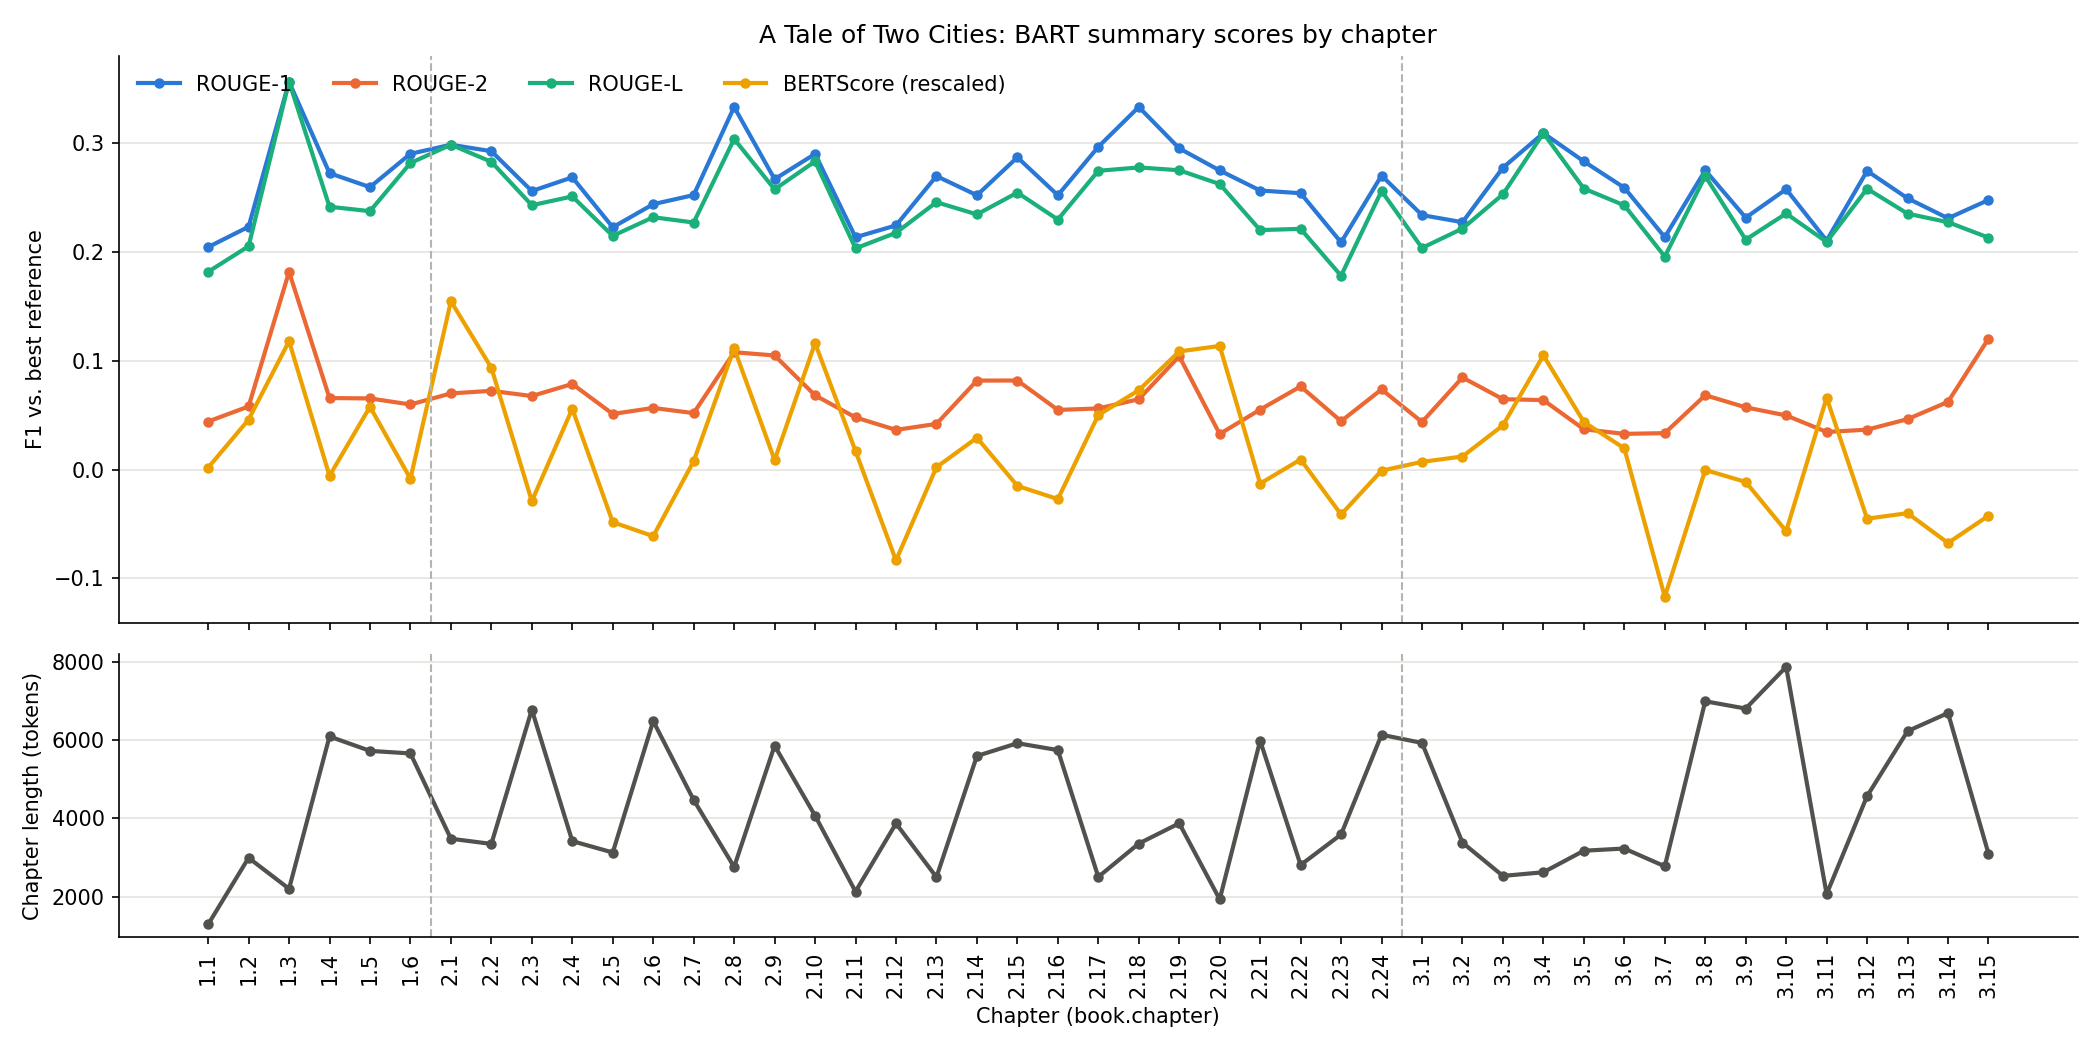
\includegraphics[width=\textwidth]{summary_scores.png}
  \caption{Summary scores by chapter (top) and chapter length in
    tokens (bottom).
  Dashed lines mark the start of Books 2 and 3.}
  \label{fig:summary}
\end{figure}

\textbf{Discussion.} BART-CNN was trained
on CNN/DailyMail
articles, where the important content is stated plainly, so it's
summarization strategy is primarily lifting sentences from the
chapter, and as such looks much closer to the prose of the book than
to anything a student might write. The BookSum references are instead written in
modern study-guide language. As such, the large gap between modern
and Dickensian English is apparant in ROUGE-2 and the BERTScore.
ROUGE-1 and ROUGE-L sit slightly above the two other metrics because
the reference and generated summaries would still share some of the
same words when referring to specific nouns or locations.

An example of a generated summary and a reference summary
demonstrates this gap very clearly, while the
generated summary
follows Dickens' sentences about the mail coach, the reference names the
characters and explains their situation. This mismatch in wording is
why the rescaled
BERTScore sits near zero. Across chapters, ROUGE barely changes with
chapter length, but BERTScore falls as chapters get longer. Longer
chapters are split into more chunks, and joining more
chunk summaries produces a choppier, less focused summary.

\textbf{Example (chapter 1.2, ``The Mail'').}

\begin{quote}\small
  \textit{Generated:} Dover road lay, as to him, beyond the Dover
  mail, as it lumbered
  up Shooter's Hill. The horses had three times already come to a
  stop, besides once
  drawing the coach across the road. The team had capitulated and
  returned to their
  duty. Three passengers were on board a coach when it was stopped by
  a guard. [\ldots]
  The rider stooped, and, casting up his eyes at the guard, handed
  the passenger a
  small folded paper.

  \textit{Reference (first of 6):} Mr. Jarvis Lorry, a confidential
  clerk at Tellson's
  Bank of London, is on his way to Dover in a mail-coach. It is a
  cold night and he is
  wrapped up to the ears, so his physical appearance is concealed from his
  fellow-passengers, all of whom are strangers. [\ldots] Jerry
  Cruncher, the rider of
  the horse, asks for Mr. Lorry, giving him a paper message [\ldots]
\end{quote}

The full per-chapter scores are in Table~\ref{tab:summary} at the end
of the report.

%-------------------------------------------------------------------------------
\section{Translation}

\textbf{Method.} The first five chapters were
translated from English to Spanish with pfnet's
plamo-3-translate-0.8b, a translation-specialized
LLM. Each chapter was split on sentence boundaries into chunks of at
most 300 words, and each chapter's chunks were translated together as
one batch. The model was run in float32 because the T4 has no native
bfloat16 support.

\textbf{Evaluation.} Each machine-translated chapter was compared
against the same
chapter of Lafuerza's translation using BLEU and chrF, from the
sacrebleu package.

\begin{table}
\caption{PLaMo 3 Translate 0.8B (English to Spanish) against Lafuerza's translation}
\label{tab:translation}
\begin{tabular}{lrrrrr}
\toprule
 & EN words & Ref. words & MT words & BLEU & chrF \\
Chapter &  &  &  &  &  \\
\midrule
1.1 & 1003 & 1185 & 1015 & 13.83 & 55.49 \\
1.2 & 2015 & 2128 & 2029 & 8.88 & 53.65 \\
1.3 & 1612 & 1665 & 1607 & 10.33 & 55.81 \\
1.4 & 4381 & 4856 & 4363 & 12.06 & 59.26 \\
1.5 & 4149 & 3843 & 4223 & 10.55 & 62.06 \\
\bottomrule
\end{tabular}
\end{table}


\textbf{Discussion.} The BLEU scores are low (mean 11.13) but chrF is moderate
(mean 57.25), this is partially because spanish is a somewhat high
morphology language (that is, the same base word can be conjugated in
different ways such that it makes a n-gram measure like BLEU fail).
chrF is also more leniant in regards to how strictly a translation
adheres to the reference, since it gives credit for similar letter sequences.

Reading the output shows the generated translations themselves are
accurate. The gap comes from the reference since Lafuerza's
translation is literary, and the LLM instead translated directly. The
opening line shows the difference clearly:

\begin{quote}\small
  \textit{English:} It was the best of times, it was the worst of
  times, it was the age
  of wisdom, it was the age of foolishness [\ldots]

  \textit{PLaMo:} Fue la mejor época, fue la peor época, fue la edad
  de la sabiduría,
  fue la edad de la necedad [\ldots]

  \textit{Lafuerza:} Erase el mejor de los tiempos y el más
  detestable de los tiempos;
  la época de la sabiduría y la época de la bobería [\ldots]
\end{quote}

The model translates the text more or less word for word, but BLEU counts exact
matches of word sequences, and the two versions rarely use the same
phrasing, since Lafuerza mimics the tone and period of Dickens.
chrF's leniancy makes it the more informative metric against a loose
reference like this one.

%-------------------------------------------------------------------------------
\section{Retrieval and Question Answering}

\textbf{Method.} Questions are answered in two steps: TF-IDF retrieval
(scikit-learn, English stop words removed, sublinear term frequency)
finds the three pieces of text most similar to the question by cosine
similarity, then an extractive reader picks an answer span from each
and the most confident one is kept. Five questions with known answers
, generated by claude code (I have not read this book) were used. To
evaluate retrieval separately from reading, if the
answer text appeared in the top 3 records whether the answer text
appears anywhere in the retrieved text. Then and whether
the final answer contains it the known correct text is recorded seperately.

The first version treated each chapter as one
document and used deepset's roberta-base-squad2 as the reader. This model is
fine-tuned for question answering questions based on short wikipedia
paragraphs. Using each chapter as the base document for TF-IDF to
retrieve resulted in the LLM answering none of the questions
correctly. This was less the fault of the reader and more of the
retrieval method, since with entire chapters the answer was buried in
too much useless information.  Instead, each chapter was
split into overlapping 200-word passages (50-word overlap), giving
909 passages. The answer span is the highest-scoring
start/end pair within the passage, up to 30 tokens long.

{\small \begin{table}
\caption{TF-IDF retrieval of the top 3 200-word passages, then answers from deepset/roberta-base-squad2}
\label{tab:qa}
\begin{tabular}{>{\raggedright\arraybackslash}p{3.3cm}>{\raggedright\arraybackslash}p{2.1cm}>{\raggedright\arraybackslash}p{2.6cm}>{\raggedright\arraybackslash}p{1.1cm}>{\raggedright\arraybackslash}p{2.4cm}>{\raggedright\arraybackslash}p{0.9cm}rl}
\toprule
Question & Expected & Top 3 passages: ch. (cos sim) & Answer in top 3 & Answer & Answer ch. & Score & Correct \\
\midrule
What is the name of the bank Mr. Lorry works for? & Tellson's & 1.4 (0.14), 3.13 (0.14), 2.3 (0.12) & True & Tellson & 2.3 & 0.50 & True \\
What number was Doctor Manette's cell in the Bastille? & One Hundred and Five, North Tower & 3.9 (0.28), 3.10 (0.15), 3.2 (0.15) & True & One Hundred and Five & 3.9 & 0.26 & True \\
Who was tried for treason at the Old Bailey? & Charles Darnay & 2.2 (0.21), 2.2 (0.17), 2.2 (0.14) & False & Mr. Jerry Cruncher & 2.2 & 0.01 & False \\
What does Madame Defarge do while she sits in the wine-shop? & knits & 2.22 (0.19), 2.15 (0.18), 2.15 (0.18) & True & taken up her knitting & 2.15 & 0.03 & True \\
Who takes Darnay's place at the guillotine? & Sydney Carton & 2.16 (0.18), 3.15 (0.10), 2.16 (0.10) & False & Spy & 3.15 & 0.00 & False \\
\bottomrule
\end{tabular}
\end{table}
}

\textbf{Discussion.} Three of the five answers were answered correctly
(``Tellson'', ``One
Hundred and Five'', ``taken up her knitting'').  The retrieved
passages are also on topic, for example, the top passage for the
Bastille question is Defarge's testimony at Darnay's trial, which names the cell
outright.

Both failures are retrieval failures; the answer is not in
any retrieved passage, so no reader could find it:
\begin{itemize}
  \item \textbf{Old Bailey.} All three passages come from the right
    chapter (2.2, the
    trial), but from its opening, where Jerry Cruncher enters the
    court before the
    prisoner has been named. The reader answered with the only person
    in the passage.
  \item \textbf{Guillotine.} The top passage matches on the words ``takes'' and
    ``place'' in Madame Defarge's line about the revolution, ``when
    it is ready, it takes
    place''. TF-IDF matches words, not meaning, and the passage that
    describes Carton's
    sacrifice (chapter 3.13) shares few words with the question.
\end{itemize}

Both wrong answers scored 0.01 or less, so a threshold around 0.02
would have rejected both instead of returning a wrong answer. With
passages, retrieval is the limiting step. Rephrasing the question
with words the book uses (``Who goes to the guillotine
in Darnay's stead?'') or a retriever that matches on meaning rather
than tokens would address the two misses.

%-------------------------------------------------------------------------------
\section{Text Generation}

\textbf{Method.} Five seeds were made from the first 20 words of five
random, lesser known chapters. Chapter 1.1 was left out because GPT-2 has
memorized its famous opening. \texttt{openai-community/\allowbreak
gpt2} generated 60 new tokens from each seed using nucleus sampling
($p = 0.9$, temperature 0.8, no repeated 3-grams, random seed 0).

\textbf{Evaluation.} Perplexity was computed by a separate, larger model,
gpt2-large, so that the generator does not grade its own
output. It scores just the generated continuation, with the seed as
context. As a baseline, the same perplexity was computed for the
book's real continuation, cut to the same number of tokens.

\begin{table}
\caption{GPT-2 continuations of 20-word seeds from the book. Perplexity is scored by GPT-2 Large on the continuation given the seed, for the generated text and for the book's own next tokens.}
\label{tab:generation}
\begin{tabular}{l>{\raggedright\arraybackslash}p{3.6cm}>{\raggedright\arraybackslash}p{7.0cm}rr}
\toprule
Ch. & Seed & Generated continuation & PPL (generated) & PPL (book) \\
\midrule
1.2 & It was the Dover road that lay, on a Friday night late in November, before the first of the persons & to enter the castle came along. "I looked over at the front of the road and noticed that the castle had been built for the war. As I approached it, the first thing that struck me was the sheer volume of prisoners. I was taken aback, but the next thing I knew & 11.54 & 46.41 \\
2.1 & Tellson’s Bank by Temple Bar was an old-fashioned place, even in the year one thousand seven hundred and eighty. It & was built at the top of the hill by the Roman Empire and was located within a large open-air church. The church was a small and imposing structure built from the ground up in the middle of a large building with a central door and windows. It is said that the building was made of wood & 13.24 & 16.10 \\
2.7 & Monseigneur, one of the great lords in power at the Court, held his fortnightly reception in his grand hotel in & Paris, with the usual welcome and attention of the guests. His visit was accompanied by a procession of about twenty-four people. All the rest were present, and the people had no idea what to expect. The receptionist was not very good, but he had a good understanding of the subject, & 16.83 & 27.18 \\
3.1 & The traveller fared slowly on his way, who fared towards Paris from England in the autumn of the year one & thousand seven hundred and eighty-seven. I would not have dared to ask him if he was alive. & 7.68 & 17.28 \\
3.5 & One year and three months. During all that time Lucie was never sure, from hour to hour, but that the & young man's spirit was still strong and that he was going to be in the best of shape. When he heard the news of Lucie's passing, he took his heart to help. (Note: This was a conversation that the family had with his brother and his sister. The & 17.30 & 90.36 \\
\bottomrule
\end{tabular}
\end{table}


\textbf{Discussion.} The generated text has a mean perplexity of 13.32, against
39.47 for Dickens' actual continuations, so GPT-2 Large finds GPT-2's text
\emph{less} surprising than the book's. As with the summarization,
this again demonstrates the large gap between modern and Dickensian
English. Since GPT-2 is trained on a primarily modern corpus, it is
reasonable that it would generate words that are more modern in nature.
Sampled text is drawn from high-probability regions of a
GPT-2 model, so a model from the same family predicts it easily.
Dickens' idiosyncratic (even for his own time) prose is far harder
to predict. Reading the output makes this clear: the
continuations are fluent but generic and drift away from the book
The largest gap is for chapter 3.5, whose real
continuation (perplexity 90.36) is written in Dickens' most
particular register. Perplexity measures how
predictable text is to a model, not how faithful or interesting it
is, so it should be read alongside the samples themselves.

%-------------------------------------------------------------------------------
\clearpage
\appendix
\section{Per-chapter summarization scores}
{\footnotesize\renewcommand{\arraystretch}{1.0}\begin{longtable}{lrrrrr}
\caption{BART-large-CNN chapter summaries scored against the best-matching BookSum reference (F1). BERTScore is rescaled with its baseline.} \label{tab:summary} \\
\toprule
 & ROUGE-1 & ROUGE-2 & ROUGE-L & BERTScore & Tokens \\
Ch. &  &  &  &  &  \\
\midrule
\endfirsthead
\caption[]{BART-large-CNN chapter summaries scored against the best-matching BookSum reference (F1). BERTScore is rescaled with its baseline.} \\
\toprule
 & ROUGE-1 & ROUGE-2 & ROUGE-L & BERTScore & Tokens \\
Ch. &  &  &  &  &  \\
\midrule
\endhead
\midrule
\multicolumn{6}{r}{Continued on next page} \\
\midrule
\endfoot
\bottomrule
\endlastfoot
1.1 & 0.205 & 0.044 & 0.182 & 0.002 & 1288 \\
1.2 & 0.223 & 0.058 & 0.205 & 0.046 & 2988 \\
1.3 & 0.357 & 0.182 & 0.357 & 0.118 & 2198 \\
1.4 & 0.272 & 0.066 & 0.242 & -0.006 & 6088 \\
1.5 & 0.260 & 0.065 & 0.238 & 0.058 & 5720 \\
1.6 & 0.290 & 0.060 & 0.282 & -0.008 & 5655 \\
2.1 & 0.299 & 0.070 & 0.299 & 0.155 & 3476 \\
2.2 & 0.293 & 0.072 & 0.283 & 0.094 & 3344 \\
2.3 & 0.256 & 0.068 & 0.243 & -0.029 & 6773 \\
2.4 & 0.269 & 0.079 & 0.251 & 0.056 & 3415 \\
2.5 & 0.223 & 0.051 & 0.215 & -0.048 & 3124 \\
2.6 & 0.244 & 0.057 & 0.232 & -0.061 & 6481 \\
2.7 & 0.252 & 0.052 & 0.227 & 0.008 & 4466 \\
2.8 & 0.333 & 0.108 & 0.304 & 0.112 & 2756 \\
2.9 & 0.267 & 0.105 & 0.258 & 0.009 & 5853 \\
2.10 & 0.290 & 0.068 & 0.283 & 0.116 & 4065 \\
2.11 & 0.214 & 0.048 & 0.203 & 0.017 & 2127 \\
2.12 & 0.224 & 0.037 & 0.218 & -0.083 & 3866 \\
2.13 & 0.270 & 0.042 & 0.246 & 0.002 & 2495 \\
2.14 & 0.252 & 0.082 & 0.235 & 0.029 & 5590 \\
2.15 & 0.287 & 0.082 & 0.255 & -0.015 & 5916 \\
2.16 & 0.252 & 0.055 & 0.230 & -0.027 & 5740 \\
2.17 & 0.297 & 0.056 & 0.275 & 0.050 & 2501 \\
2.18 & 0.333 & 0.065 & 0.278 & 0.073 & 3352 \\
2.19 & 0.295 & 0.104 & 0.275 & 0.109 & 3870 \\
2.20 & 0.275 & 0.033 & 0.262 & 0.114 & 1928 \\
2.21 & 0.257 & 0.055 & 0.220 & -0.013 & 5980 \\
2.22 & 0.254 & 0.077 & 0.221 & 0.009 & 2805 \\
2.23 & 0.209 & 0.045 & 0.178 & -0.041 & 3585 \\
2.24 & 0.270 & 0.074 & 0.256 & -0.001 & 6132 \\
3.1 & 0.234 & 0.044 & 0.204 & 0.007 & 5923 \\
3.2 & 0.227 & 0.085 & 0.222 & 0.012 & 3376 \\
3.3 & 0.278 & 0.065 & 0.253 & 0.041 & 2526 \\
3.4 & 0.309 & 0.064 & 0.309 & 0.105 & 2620 \\
3.5 & 0.283 & 0.037 & 0.258 & 0.044 & 3170 \\
3.6 & 0.259 & 0.033 & 0.243 & 0.020 & 3226 \\
3.7 & 0.214 & 0.034 & 0.196 & -0.117 & 2771 \\
3.8 & 0.275 & 0.068 & 0.270 & -0.000 & 6987 \\
3.9 & 0.232 & 0.057 & 0.211 & -0.011 & 6801 \\
3.10 & 0.258 & 0.050 & 0.235 & -0.057 & 7866 \\
3.11 & 0.211 & 0.035 & 0.209 & 0.066 & 2062 \\
3.12 & 0.275 & 0.037 & 0.258 & -0.045 & 4565 \\
3.13 & 0.249 & 0.046 & 0.235 & -0.040 & 6224 \\
3.14 & 0.231 & 0.062 & 0.227 & -0.067 & 6687 \\
3.15 & 0.248 & 0.120 & 0.213 & -0.042 & 3095 \\
\end{longtable}
}

\clearpage
\section{Code}
\inputminted[
  fontsize=\footnotesize,
  linenos,
  breaklines,
  frame=lines,
]{python}{assignment4.py}

\end{document}
